\documentclass[usenames,dvipsnames]{beamer}
% \usepackage[noend]{algorithmic}
% \usepackage{paralist}
\usepackage{latexsym,amsmath,url}
\usepackage{hyperref}
\usepackage{color}
\DeclareSymbolFont{AMSb}{U}{msb}{m}{n}
\DeclareMathSymbol{\N}{\mathbin}{AMSb}{"4E}
\DeclareMathOperator*{\argmax}{argmax}

\newcommand{\vecb}[1]{\mathbf{#1}}
\newcommand{\x}{\mathbf{x}}
\newcommand{\y}{\mathbf{y}}
\newcommand{\w}{\mathbf{w}}
\newcommand{\z}{\mathbf{z}}
\newcommand{\X}{\mathbf{X}}
\newcommand{\Y}{\mathbf{Y}}
\newcommand{\Z}{\mathbf{Z}}
\newcommand{\voc}[1]{\emph{\color{ForestGreen}#1}}

\newcommand{\superscript}[1]{\ensuremath{^\textrm{\scriptsize#1 }}}
\mode<presentation>{ 
  \usetheme{Boadilla}
  %\setbeamercovered{invisible}
  % or whatever (possibly just delete it)
} \title[ML / NLP Course ]{Sequence Labeling}


\author[Chrupala and Stroppa]{Grzegorz Chrupa{\l}a and Nicolas Stroppa}

\institute[]  % (optional, but mostly needed)
{
Saarland University\\
Google
}
\date[2010] % (optional, should be abbreviation of conference name)
{META Workshop}


\pgfdeclareimage[height=1cm]{UdS}{SaarlandUniversityLogo.jpg}
% \logo{\pgfuseimage{UdS}}

\AtBeginSection[]
 {
    \begin{frame}
        \frametitle{Outline}
        \tableofcontents[currentsection]
    \end{frame}
 }
\begin{document}
\frame{\titlepage}

\begin{frame}
  \frametitle{Outline}
  \tableofcontents
\end{frame}

\section{Conditional Random Fields}
\begin{frame}\frametitle{Context}

Sequence labeling setting:
\begin{itemize}
\item Input sequence: $\x = x_1, x_2, \dots, x_N$
\item Output sequence: $\z = z_1, z_2, \dots, z_N$
\end{itemize}

\vspace{0.4cm}
Methods already introduced for sequence labeling: HMM (generative), Maximum Entropy Markov
Model (discriminative)

\end{frame}

\begin{frame}\frametitle{Example}

\begin{center}
\begin{tabular}{ccc|c}
\hline
Word & POS & Chunk & NE \\
\hline
West & NNP & B-NP & B-MISC \\
Indian & NNP & I-NP & I-MISC \\
all-rounder & I-NP & B-NP & O \\
Phil & NNP & I-NP & B-PER \\
Simons & NNP & I-NP & I-PER \\
took & VBP & B-VP & O \\
four & CD & B-NP & O \\
for & IN & B-PP & O \\
38 & CD & B-NP & O \\
on & IN & B-PP & O \\
Friday & NNP & B-NP & O \\
as & IN & B-PP & O \\
Leicestershire & NNP & B-NP & B-ORG \\
beat & VBP & B-VP & O \\
\end{tabular}
\end{center}

\end{frame}

\begin{frame}\frametitle{Discriminative models for Sequence Labeling -
  Local classifier}

For each position $i$, classify each $x_i$ independently (sliding window)
\begin{itemize}
\item Criterion: $z_i = \argmax P(z_i|x_i)$
\item Each example consists of a single position in the sequence (a token/label pair)
\item Any classification algorithm can be used \pause
\begin{itemize}
\item Maxent
\item Perceptron
\item k-nn
\item SVM
\item \dots
\end{itemize}
\end{itemize}

\pause
\vspace{0.4cm}
Problem: the sequence nature of the problem is not taken into account
at all (e.g.\ nothing preventing from outputing impossible label bigrams)
\end{frame}

\begin{frame}\frametitle{Discriminative models for Sequence Labeling -
  Local classifier++}

Local classifier with previous labels: for each position $i$, classify
each $x_i$ sequentially (e.g.\ from left to right), making use of the previously assiged label
\begin{itemize}
\item Criterion: $z_i = \argmax P(z_i|x_i, z_{i-1})$
\item Training is performed similarly as before, but we now can design
  features that include the previous label
\end{itemize}

\pause
\vspace{0.4cm}
Problem: Errors can be easily propagated

\end{frame}


\begin{frame}\frametitle{Discriminative models for Sequence Labeling -
  MEMM}

Maximum entropy Markov Model: same as above for training, but label by maximizing on the entire sequence
\begin{itemize}
\item $z = \argmax P(\z|\x) = \argmax \Pi_i P(z_i|x_i, z_{i-1})$
\end{itemize}

\pause
\vspace{0.4cm}
Problem: we're learning a model on a position-basis, so we're
  still not fully exploiting the sequential nature of the data

\end{frame}



\begin{frame}\frametitle{Conditional Random Fields}

\voc{Conditional Random Fields} enable to define ``true'' sequence learning
models, i.e.\ models that learn and operate on sequences.

\vspace{0.4cm}
This means we model directly
\begin{equation*}
P(\z|\x)
\end{equation*}
without resorting to position-based decompositions of the model definition.

\vspace{0.4cm}
As they are able to deal \emph{natively} with ``structured'' data, they are
referred to as \voc{structure learning} methods.
\end{frame}


\begin{frame}\frametitle{Conditional Random Fields}
Some reasons to focus on CRFs.
\begin{itemize}
\item \emph{Sound} and understood principle (maximum entropy)
\item Very \emph{flexible} for feature definition
\item \emph{Natively'} handling sequences
\item \emph{State of the art results} on numerous applications
\item Because of this success, now the \emph{baseline} in sequence
  labeling
\end{itemize}

\end{frame}

\begin{frame}\frametitle{Conditional Random Fields}

\begin{itemize}
\item The principles underlying Conditional Random Fields are identical to
the one behind Maximum Entropy classifiers
\item You can actually view CRFs as the counterpart of Maxent for
  sequences
\end{itemize}

\pause
This yields the following model:
\vspace{0.4cm}
\begin{equation*}
P(\z|\x) = \frac{\exp(\w . \Phi(\x,\z))}{Z(\x)},
\end{equation*}
where $Z(\x) = \sum_z \exp(\w . \Phi(\x,\z))$ is the partition function.

\vspace{0.4cm}
Remarks:
\begin{itemize}
\item Features now operate on sequences
\item The sum in the partition function is big!
\end{itemize}

\end{frame}

\begin{frame}\frametitle{Conditional Random Fields as a linear model}

CRF model:
\begin{equation*}
P(\z|\x) = \frac{\exp(\w . \Phi(\x,\z))}{Z(\x)}
\end{equation*}

\vspace{0.4cm}
CRF prediction:
\begin{align*}
\argmax_z P(\z|\x) &= \argmax \frac{\exp(\w . \Phi(\x,\z))}{Z(\x)} \\
                               &= \argmax \exp(\w . \Phi(\x,\z)) \\
                               &= \argmax \w . \Phi(\x,\z)
\end{align*}

\vspace{0.4cm} Once the model is learnt, it's a basic linear model, so
you can \emph{apply} the model the same way as for MeMM or structured
perceptron...

\end{frame}

\begin{frame}\frametitle{Linear Conditional Random Fields Features}

General form: $\Phi_j(\x,\z)$

\vspace{0.4cm}
In linear CRFs, we assume a particular structure (close to HMM).

\vspace{0.4cm}
Features are the same as for MeMM, or structured perceptron\dots


\end{frame}



\begin{frame}\frametitle{Training Conditional Random Fields}

How do we train CRFs?

\vspace{0.4cm}
No closed form to the associated optimization problem.  Needs to
resort to numeric optimization techniques:
\begin{itemize}
\item L-BFGS
\item Improved Iterative Scaling
\item Stochastic Gradient Descent (SGD)
\end{itemize}

\vspace{0.4cm}
We'll focus on SGD since it's quite easy, efficient and we already mentionned it
\end{frame}


\begin{frame}\frametitle{Stochastic Gradient Descent}

Expression of the \voc{conditional log-likelihood}:
\begin{equation*}
  \log P(\z|\x;\w) = \log \frac{\exp(\w . \Phi(\x,\z))}{\sum_{z'}
    \exp(\w. \Phi(\x,\z'))} = \w . \Phi(\x,\z)- \log \sum_{z'} \exp(\w . \Phi(\x,\z'))
\end{equation*}
Our goal is to \emph{maximize} this likelihood.

\vspace{0.4cm}
In order to perform gradient descent, we need to compute its gradient.
\begin{align*}
\nabla_\w \log P(\z|\x;\w) &= \Phi(\x,\z)- \sum_{z'} \Phi(\x,\z') \frac{\exp(\w
  . \Phi(\x,\z'))}{\sum_{z'}' \exp(\w. \Phi(\x,\z''))} \\
                                          &= \Phi(\x,\z)- \sum_{z'}
                                          \Phi(\x,\z') P(\z'|\x;\w) \\
                                          &= \Phi(\x,\z)- E_{P(\z'|\x;\w)} \Phi(\x,\z')
\end{align*}
\end{frame}


\begin{frame}\frametitle{Stochastic Gradient Descent}
In stochastic gradient descent, we appromixate this conditional
log-likelihood with the \voc{empirical} conditional
log-likelihood, computed on training examples.
\begin{equation*}
\nabla_\w \log P(\Z|\X;\w) = \sum_i \Phi(\x_i,\z_i)- E_{P(\z'_i|\x_i;\w)} \Phi(\x_i,\z_i')
\end{equation*}

\vspace{0.4cm}
The idea is that we sample the example, and apply an update rule per example:
\begin{equation*}
 \w \leftarrow \w + \Phi(\x_i,\z_i)- E_{P(\z'_i|\x_i;\w)} \Phi(\x_i,\z_i')
\end{equation*}

\vspace{0.4cm}
Note: computation of $E_{P(\z'_i|\x_i;\w)} \Phi(\x_i,\z_i')$ can be done by
dynamic programming if we use linear CRF (cf. forward-backward algo).
\end{frame}

\begin{frame}\frametitle{Some notes on SGD}
SGD only computes the gradient (first-order partial derivatives), and not the hessian
(second-order partial derivatives).

\vspace{0.4cm}
Using the first-order info is less precise but it's much more efficient than using
second-order info.

\vspace{0.4cm}
There exists some more or less complex improvements made around this
to keep this efficient while making it less approximative.
\end{frame}


\section{Additional Remarks}

\begin{frame}\frametitle{Structured perceptron}

CRF SGD update:
\begin{equation*}
 \w \leftarrow w + \Phi(\x_i,\z_i)- E_{P(\z'_i|\x_i;\w)} \Phi(\x_i,\z_i')
\end{equation*}

\vspace{0.4cm}
Structured perceptron update:
\begin{equation*}
 \w \leftarrow w + \Phi(\x_i,\z_i)- \Phi(\x_i,\hat{\z}_i'),
\end{equation*}
with:
\vspace{0.4cm}
\begin{equation*}
E_{P(\z'|\x;\w)} \Phi(\x,\z') = \sum_{z'} \Phi(\x,\z') \frac{\exp(\w . \Phi(\x,\z'))}{\sum_{z'}' \exp(\w. \Phi(\x,\z''))} 
\end{equation*}
and
\begin{equation*}
\Phi(\x_i,\hat{\z}_i') = \sum_{z'} \Phi(\x,\z') (1 if z' is best output, 0 otherwise).
\end{equation*}

\vspace{0.4cm}
The only difference is that CRF SGD is using softmax and structured
perceptron ``hard'' max!
\end{frame}


\begin{frame}\frametitle{Comparison with HMM and Maxent}

\begin{block}{Analogy}
If you make sense of the following analogy, we're quite happy!
\begin{center}
  Maxent:Naive Bayes::CRF::HMM
\end{center}
\end{block}

\pause
\begin{center}
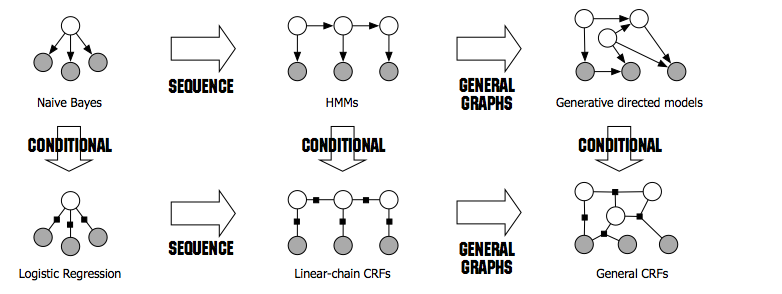
\includegraphics[scale=0.4]{crfanalogy}
\end{center}

\end{frame}

\begin{frame}\frametitle{Linear and higher-order CRF}
  There exists several ``flavors'' of CRF, with different
  expressiveness power.
\end{frame}

\begin{frame}\frametitle{Semi-markov CRF}
In semi-markov CRFs, we can define features on several consecutive
positions (segmentation as a hidden variable).

Input and Output sequences can have different length.
\end{frame}
%  ... Regularization...

\end{document}

